
% Preamble
\documentclass{assignment}

% Packages
\usepackage{minted}
\usepackage{dsfont}
\usepackage{colortbl}
\usepackage[linesnumbered,ruled,longend]{algorithm2e} \usepackage[colorlinks=true,linkcolor=blue]{hyperref}
\usepackage{forest}
\usepackage{multirow}

\SetKwInOut{Input}{Input} \SetKwInOut{Output}{Output} \SetKwProg{Fn}{Function}{\string:}{end} \SetKwFunction{algohw}{AlgoHw}
\SetKwFunction{algo}{FindRamanujam}
% Document
\begin{document}

    \maketitle

    \newpage

	% Q1
    \begin{homeworkProblem}
\begin{center}
\textbf{Fast multi-point evaluation}
\end{center}    
    
\begin{enumerate}
\item The binary tree by splitting $U$ is 

\begin{center}
    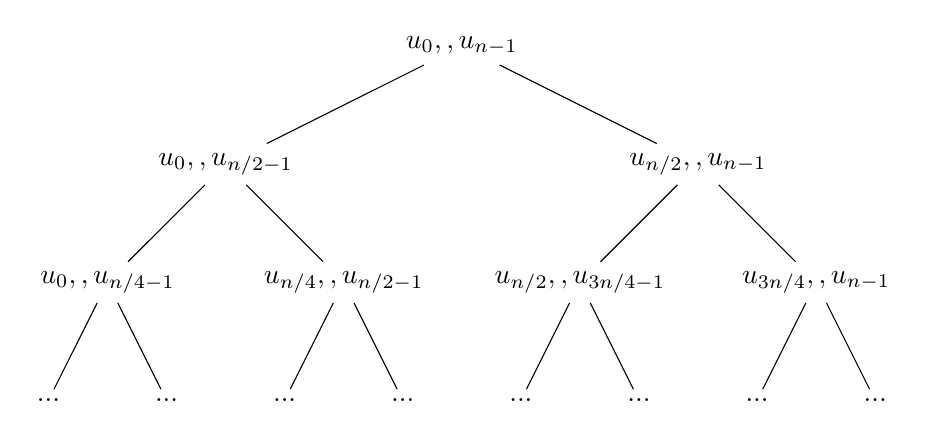
\begin{tikzpicture}
 \node {$u_0, \dotsb ,u_{n-1}$}
 child {node {$u_0, \dotsb ,u_{n/2-1}$}
  child {node {$u_0, \dotsb ,u_{n/4-1}$}
   child {node {...}}
   child {node {...}}
  }
  child [missing] {}
  child {node {$u_{n/4}, \dotsb ,u_{n/2-1}$}
   child {node {...}}
   child {node {...}}
  }
 }
 child [missing] {} 
 child [missing] {}
 child [missing] {} 
 child {node {$u_{n/2}, \dotsb ,u_{n-1}$}
  child {node {$u_{n/2}, \dotsb ,u_{3n/4-1}$}
   child {node {...}}
   child {node {...}}
  }
  child [missing] {}
  child {node {$u_{3n/4}, \dotsb ,u_{n-1}$}
   child {node {...}}
   child {node {...}}
  }
 };
 \end{tikzpicture}
 \end{center}

\item From $M_{i,j}=\prod_{l=0}^{2^i-1}m_{j2^i+l}$
\begin{align*}
M_{i+i,j}&=\prod_{l=0}^{2^{i+1}-1}m_{j2^{i+1}+l}\\
&= \prod_{l=0}^{2^{i}-1}m_{j2^{i+1}+l} \cdot \prod_{l=2^i}^{2^{i+1}-1}m_{j2^{i+1}+l} \\
&= \prod_{l=0}^{2^{i}-1}m_{2j2^{i}+l} \cdot\prod_{l=0}^{2^i-1}m_{(2j+1)2^i+l} \\
&=M_{i,2j} \cdot M_{i,2j+1}\\[2ex]
M_{0,j}&=\prod_{l=0}^{2^0-1}m_{j2^0+l} =m_j
\end{align*}
\item The polynomial $M_{i,j}$ represents that for the node at height $k-i$, $j$ nodes from left, the product of all the leaves underneath. As each leaf represents $M_{0,j}=x-u_j$. 

\begin{center}
    \begin{tikzpicture}
 \node {$M_{k,0} \prod_{i=1}^{n-1}(x-u_i)$}
 child {node {$M_{k-1,0} \prod_{i=1}^{n/2-1}(x-u_i)$}
  child {node {...}
   child {node {$M_{0,0}=(x-u_{0})$}}
   child {node {...}}
  }
  child [missing] {}
  child {node {...}
   child {node {...}}
   child {node {...}}
  }
 }
 child [missing] {} 
 child [missing] {}
 child [missing] {} 
 child {node {$M_{k-1,1} \prod_{i=n/2}^{n-1}(x-u_i)$}
  child {node {...}
   child {node {...}}
   child {node {...}}
  }
  child [missing] {}
  child {node {...}
   child {node {...}}
   child {node {\qquad \qquad $M_{0,n-1}=(x-u_{n-1})$}}
  }
 };
 \end{tikzpicture}
 \end{center}
     
\item 
a) 
 
\begin{algorithm}[H]
\Input{$n=2^k$, $k\in \mathbb{N}$. $u_0,\dots,u_{n-1}\in R$}
\Output{$M_{i,j}$ for $1\leq i \leq k$ and $0\leq j < 2^{k-i}$} \BlankLine
\For {$j \leftarrow 0$ \KwTo $n-1$} {
$M_{0,j} \leftarrow (x-u_i)$ \\
}
\For {$i \leftarrow 1$ \KwTo $k$}{
	\For {$j \leftarrow 0$ \KwTo $2^{k-i}-1$} {
		$M_{i,j} \leftarrow M_{i-1,2j} \cdot M_{i-1,2j+1}$	
	}
}
\KwRet{$M_{i,j}$} 
\caption{Build up the subproduct tree} \end{algorithm}

b)
 
\begin{algorithm}[H]
\Input{$n=2^k$, $k\in \mathbb{N}$. $P\in R[x]$ of degree less than $n$. $u_0,\dots,u_{n-1}\in R$. subproducts $M_{i,j}$}
\Output{$P(u_0), P(u_1),\dots , P_{u_{n-1}} \in R$} \BlankLine
\If {$n==1$} {\KwRet{$P\in R$}}
$A_0 \leftarrow P$ mod $M_{k-1,0}$ \\
$A_1 \leftarrow P$ mod $M_{k-1,1}$ \\
$A_0(u_0),\dots ,A_0(u_{n/2-1}) \leftarrow$ call algorithm with input $A_0,n/2$, subtree rooted at $M_{k-1,0}$ \\
$A_1(u_{n/2}), \dots ,A_1(u_{n-1}) \leftarrow$ call algorithm with input $A_1,n/2$, subtree rooted at $M_{k-1,1}$ \\
\KwRet{$A_0(u_0),...,A_0(n/2-1),A_1(u_{n/2}),..., A_1(u_{n-1})$} 
\caption{Go down the subproduct tree} \end{algorithm}

\item 
\begin{enumerate}

\item[a)] Proof by induction 

When $k=0$, \textbf{Algorithm 2} will return at line 2 directly,which satisfies the hypothesis. 

When $k \geq 1$, evaluate $P$ at $u_i$. Assume $q_0$ as the quotient of $P$ divided by $M_{k-1,0}$ and $q_1$ be the quotient of $P$ divided by $M_{k-1,1}$. 

Then it gives 
\begin{equation*}
P(u_i) \begin{cases}
q_0(u_i)\cdot M_{k-1,0}(u_i) + A_0(u_i)=A_0(u_i) \quad \text{if } 0\leq i < n/2 \\
 q_1(u_i)\cdot M_{k-1,1}(u_i) + A_1(u_i)=A_1(u_i) \quad \text{if } n/2\leq i < n
\end{cases}
\end{equation*}

\item[b)] 
$$T(n)=2T(n/2) + O(M(n))$$
From Master Theorem, the time complexity is $\mathcal{O}(M(n)\text{log}n)$


\end{enumerate}
\end{enumerate}
\newpage
\begin{center}
\textbf{Fast interpolation}
\end{center}  

\begin{enumerate}
\item 
Give distinct $u_0,\dots, u_{n-1} \in R$ and the arbitrary $v_0,\dots, v_{n-1}$ in a field $F$, Lagrange interpolation says that the unique polynomial $P\in F[x]$ which solves the 
$$P(u_0),\dots, P(u_{n-1})=(v_0,\dots, v_{n-1})$$
takes the form $$P=\sum_{0\leq i < n} v_is_i\frac{m}{(x-u_i)},$$
where $m=(x-u_0)\cdots (x-u_{n-1})$ and 
$$s_i=\prod_{j\neq i} \frac{1}{u_i - u_j}$$

\item 
$$m^{'} = \left( \prod_{i=0}^{n-1}(x-u_i) \right)^{'} = \sum_{i=0}^{n-1} (x-u_i)^{'} \frac{m}{x-u_i} = \sum_{i=0}^{n-1} \frac{m}{x-u_i}$$ 
$\frac{m}{x-u_i}$ vanishes at all points $u_j$ with $i\neq j$, so 
$$m^{'}(u_i)=\frac{m}{x-u_i}|_{x=u_i}=\frac{1}{s_i}$$
\item Algorithm 

\begin{algorithm}[H]
\Input{$n=2^k$, $k\in \mathbb{N}$. $u_0,\dots,u_{n-1}\in R$, subproducts $M_{i,j}$ for $1\leq i \leq k$ and $0\leq j < 2^{k-i}$}
\Output{$P(u_0), P(u_1),\dots , P_{u_{n-1}}$} \BlankLine
\If {$n==1$} {\KwRet{$P\in R$}}
$left \leftarrow$ call algorithm with input $k-1, 2i$\\
$right \leftarrow$ call algorithm with input $k-1,2i+1$\\
\KwRet{$left \times M_{k,1} + right\times M_{k,0}$} 
\caption{Interpolation} \end{algorithm}

\item 
\begin{enumerate}
\item[a)]
\item[b)] $s_i$ could be computed by evaluating $m^{'}$ at the $n$ evaluation points $u_0,\dots, u_{n-1}$. which could be done in $\O(M(n)\text{log}n)$ .
\item[c)] Once the $s_i$ is computed, the polynomial to solve the problem is created. To output a polynomial of the form $P(x)=a_0+a_1x+\dots a_{n-1}x^{n-1}$, the subproduct tree will be used to compute the sum. Then from the previous discussion, we could know the time complexity is $\O(M(n)\text{log}n)$ .
\end{enumerate}
\item It is possible because we could retrieve polynomials from the precomputed tree. 
\end{enumerate}
    
    
    \end{homeworkProblem}

\newpage
    
    % Q2
    \begin{homeworkProblem}

\begin{enumerate}
\item
\item 
\begin{itemize}
\item \textbf{$S_2:$}``No idea what those two numbers could be...” \\
The only way of taking $xy$ student to know the two numbers directly is that the product could only be decomposed into two prime numbers. Such as $15=3\times 5$. Then conclude that $xy$ is not a unique result of two prime numbers. 
\item \textbf{$S_1:$}  ``I’m not surprised, I knew you couldn’t know!” \\
For student taking $x+y$, he knows the only way for another student to know the two numbers  is two prime numbers product. Then conclude that $x+y$ could not be decomposed into two prime numbers. Then all the even numbers could be ignored. The remaining odd numbers that satisfy this condition could be generated by program: $11, 17, 23, 27, 29, 35, 37, 41, 47, 53$
\item \textbf{$S_2:$}``Uhm...so now I know...” \\
At this points, $S_2$ knows $x+y$ must be in the above list. 
\item \textbf{$S_1:$}  ``So do I!” \\
For $S_1$ to know the number, the sum must only corresponds to only one possible solution. 
\end{itemize}
Then $x=4, y=13$.
\end{enumerate}
    
    \end{homeworkProblem}
    





\end{document}
